\documentclass[12pt]{article}
\usepackage{amsfonts,amsmath,amssymb, listings}

\usepackage[utf8]{inputenc}
\usepackage{graphicx}
\usepackage{multirow}
\usepackage{xcolor}

\usepackage{threeparttable}
\usepackage{blindtext}


\usepackage[a4paper, total={6in, 8in}]{geometry}

\usepackage[numbered,framed]{matlab-prettifier}
%\usepackage{color}

%\setcounter{MaxMatrixCols}{10}

\def\stackunder#1#2{\mathrel{\mathop{#2}\limits_{#1}}}%

\newcommand{\fiid}{\func{i.i.d.}} % use this as in: X_i \stackrel{\fiid}{\sim} \func{Exp} \left( \lambda \right)
\DeclareMathOperator{\Norm}{N}

\newcommand{\platzo}{\vspace*{2cm}}
\newcommand{\platzt}{\vspace*{4cm}}

\newcommand{\findep}{\func{ind}}  % could use indep instead if ind, but 1st book uses ind.

\newcommand{\R}{\ensuremath{{\mathbb R}}}
\newcommand{\N}{\ensuremath{{\mathbb N}}}
\def\QATOP#1#2{{#1 \atop #2}}
\def\QTATOP#1#2{{\textstyle {#1 \atop #2}}}
\def\QDATOP#1#2{{\displaystyle {#1 \atop #2}}}
\voffset=-2.54cm\hoffset=-2.54cm \textheight27cm \textwidth17.0cm \topmargin0.5cm
\oddsidemargin2.00cm \evensidemargin2.00cm \unitlength1cm

\def\func#1{\mathop{\rm #1}}%
\def\dint{\mathop{\displaystyle \int}}%
\newcommand{\Ind}{\ensuremath{{\mathbb I}}} % indicator function
\newcommand{\E}{\ensuremath{{\mathbb E}}} % expected value
\newcommand{\Var}{\ensuremath{{\mathbb V}}} % variance

\setlength{\parindent}{0pt}

\usepackage{float}

\newfloat{Program}{thp}{lop}[section]
\floatname{Program}{Program Listing}

\begin{document}

\pagestyle{empty}

\bigskip

\begin{figure}[htp]
    \centering
    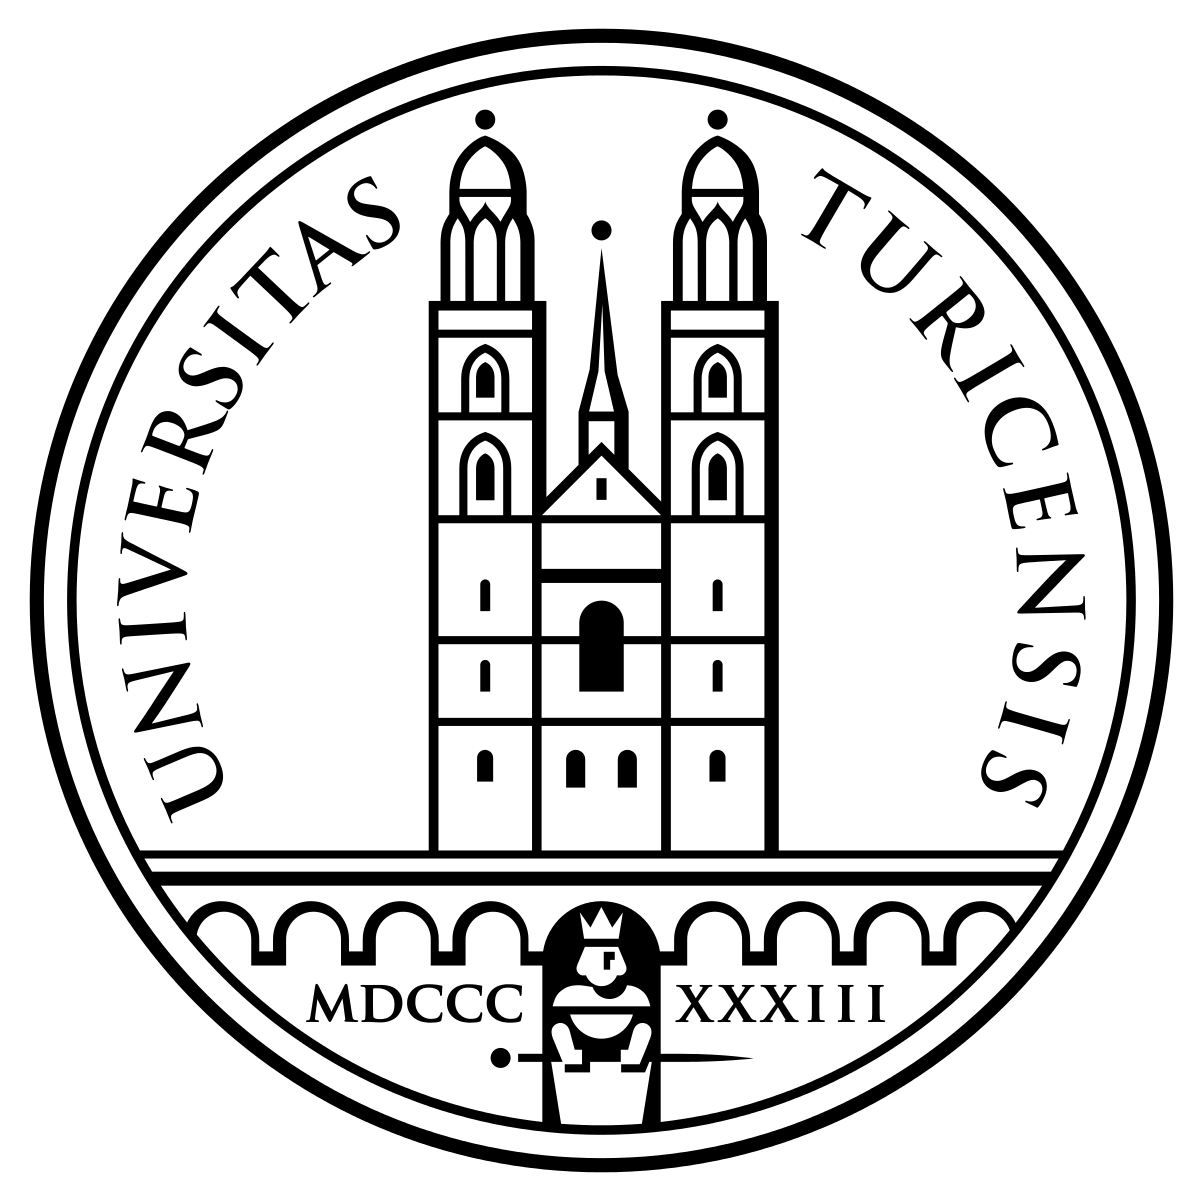
\includegraphics[width=4cm]{uzh logo 2.png}
    \label{fig:UZH}
\end{figure}

\begin{Large}
	\begin{center}
		\textbf{Digital Tools for Finance}
	\end{center}
\end{Large}

\vspace{2cm}

\begin{large}	
	\begin{center}
		\textbf{Effect of Interest Rate Changes on Cryptocurrencies} \vspace{0.1cm} \\ {Prof. Igor Pozdeev } \vspace{2cm} \\ \textbf{Matthias Olieslagers - 22714034}  \\ \textbf{
Cameron Storey - 22740815} \\
        \textbf{Marc David Parker - 22727762}\\
        \textbf{Qian Chen - 21742226}\\
	\end{center}
\end{large}

\tableofcontents

\newpage

\bigskip
\section{Introduction}

The goal of this research report is to discover how changes in FED interest rates have an impact on the prices of cryptocurrencies (e.g. Bitcoin) \newline
The up-front hypothesis, based on our knowledge of the financial markets is that the higher the FED interest rate goes, the lower the crypto prices will drop, i.e. they have a negative correlation. In this report, an attempt will be made to  confirm (or invalidate) the hypothesis statement above. \newline
In the first section, the different data sources will be covered. What does the data exactly represent and why is it relevant to look into for this particular research. In the second part, the methodology will be laid out. Lastly, the results will be critically evaluated and interpreted and a final conclusion will be provided. 

\section{Data}

The datasets that were used to develop an answer to this research question are the BTC-USD Daily Price and the FED rate, both over the extensive time period from 2016 to date. At first, we also looked at several other currencies such as Solana and the Dogecoin, but decided not to include them in the final analysis as their values are less representative for the market. We also looked at other interest rate metrics, such as the LIBOR and SOFR rate. These two interest rates relatively close follow the path of the FED rate and they are both continuous rates. All of the data was obtained from reliable sources such as Yahoo Finance and MarketWatch.

\begin{Program}[!htb]
\begin{lstlisting}[style=Matlab-editor,basicstyle=\mlttfamily\footnotesize]
dummy
  
\end{lstlisting}
\caption{Dummy code}
\label{Dummy code}
\end{Program}

\section{Explanation about the first notebook 'Analysis'}
\subsection{Methodology}
In this paragraph, we will dig deeper on the methodology for the analysis and explain and interpret the results. The extensive explanation (e.g. all of the underlying code, plots etc.) can be found in the Jupyter notebook, this report serves as a brief summary of the main findings. \newline \newline
The programming language Python, with extensions pandas, numpy and matplotlib, is used and the following approach is used. First, we read in the BTC and FED data and some of the functions for the calculation of metrics such as the Moving Average and Rolling Volatily are defined. These metrics will be used in the analysis later on. Next, the particular dates at which there was effectively a change in the FED rate are highlighted and sorted out, we will obviously focus on these particular dates when assessing what the effect of an interest change on the crypto prices is. \newline
\newline As an illustration, the graph below (see Figure \ref{fig:FED Rate evolution 2016 - 2022}) illustrates the evolution of the FED rate across the last 6 years. As can be seen, this is a stepwise function, so there are no daily changes but rather periodical changes with flat periods in between. \newline It is interesting to note that the macro-economic events can clearly be seen in the graph. At the beginning of 2020, the interest rate drops to a low point in order to support the economy during the Covid-19 outbreak. Now since the beginning of 2022, the interest rate has started to rise sharply in order to slow down the inflation. The FED rate is thus a tool to regulate the economy and in the next paragraph down below we will discuss whether these changes have any significant impact on the prices of BTC.

\begin{figure}[!htb]
   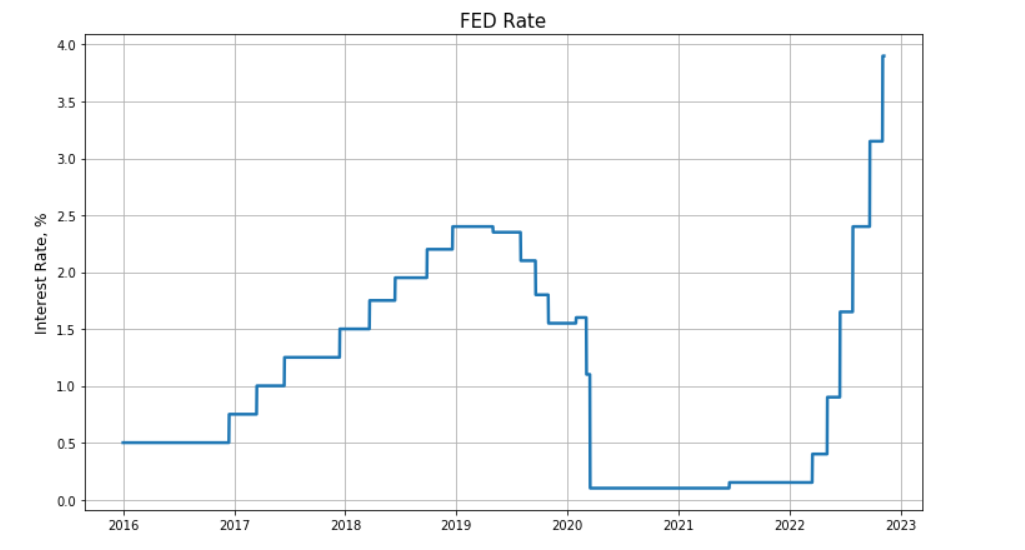
\includegraphics[scale=0.7]{research_project/text/paper/FED rate graph.png}
   \centering
   \caption{FED Rate evolution 2016 - 2022}
   \label{fig:FED Rate evolution 2016 - 2022}
\end{figure}


\subsection{Results}

\newpage
\section{Explanation about the second notebook (optional)}
Can be very short or skip this
\section{Conclusion}

\end{document}
